% This is samplepaper.tex, a sample chapter demonstrating the
% LLNCS macro package for Springer Computer Science proceedings;
% Version 2.21 of 2022/01/12
%
\documentclass[runningheads]{llncs}
%
\usepackage[T1]{fontenc}
% T1 fonts will be used to generate the final print and online PDFs,
% so please use T1 fonts in your manuscript whenever possible.
% Other font encondings may result in incorrect characters.
%
\usepackage{graphicx}
\usepackage{subcaption}
\usepackage{amsmath,amssymb}
\usepackage{hyperref}
% Used for displaying a sample figure. If possible, figure files should
% be included in EPS format.
%
% If you use the hyperref package, please uncomment the following two lines
% to display URLs in blue roman font according to Springer's eBook style:
\usepackage{color}
\renewcommand\UrlFont{\color{blue}\rmfamily}
% \usepackage{listings}
\usepackage{listingstyle}
\usepackage[inline]{enumitem}
\usepackage{tabularx}
\usepackage{formalism}
\usepackage{import}
\usepackage{xcolor}
\usepackage{todonotes}
\usepackage{cleveref}
\usepackage[firstpage]{draftwatermark}

\newcommand{\ourLang}{\textsc{ScalaTropy}}
\newcommand{\code}[1]{\lstinline[style=scala3,basicstyle=\ttfamily\small\color{vscLightText}]{#1}}
\newcommand{\diff}[1]{{#1}}
% \newcommand{\diff}[1]{{\color{magenta} #1}}

\graphicspath{{figures/}}

\begin{document}
%
\SetWatermarkText{%
  \hspace*{3.7in}%
  \raisebox{8.55in}{%
    \href{https://eapls.org/pages/artifact_badges/}{%
      \mbox{%
        
\includegraphics[width=1.4cm]{./badges/available}%
        
\includegraphics[width=1.4cm]{./badges/functional}%
      }%
    }%
  }%
}
\SetWatermarkAngle{0}
%
\title{\ourLang{}: Multiparty Coordination with Monadic Communication Primitives}
\titlerunning{\ourLang{}: Multiparty Coordination via Monads}
%
%\titlerunning{Abbreviated paper title}
% If the paper title is too long for the running head, you can set
% an abbreviated paper title here
%
\author{Nicolas Farabegoli\inst{1} \and Luca Tassinari\inst{1} \and
Gianluca Aguzzi\inst{1} \and Mirko Viroli\inst{1}}
%
\authorrunning{N. Farabegoli et al.}
% First names are abbreviated in the running head.
% If there are more than two authors, 'et al.' is used.
%
\institute{University of Bologna, Bologna, Italy\\
\email{
  \{nicolas.farabegoli,gianluca.aguzzi,mirko.viroli\}@unibo.it\\
  luca.tassinari10@studio.unibo.it
  }
}
%
\maketitle              % typeset the header of the contribution
%
\begin{abstract}
Multiparty languages 
 provide a concrete foundation for expressing complex coordination behaviors in a single, coherent specification.
%
Based on this idea, several paradigms have been proposed in the literature over the years.
%
Among them, choreographic programming is a widely adopted paradigm for defining deadlock-free distributed systems,
 while multitier programming takes a different approach, 
 focusing on partitioning system logic across different execution tiers.
%
%However, current choreographic and multitier languages have no differentiated communication primitives, causing both performance overhead and usability problems when defining distributed behavior.

Recognizing that these paradigms share fundamental similarities as multiparty languages,
we build on choreographic programming while importing static architectural descriptions and placement types inspired by ScalaLoci. % to overcome some of their limitations.
%
We introduce \ourLang{}, 
 a coordination language that integrates multiple communication schemes to establish both isotropic and anisotropic communication patterns,
 while incorporating placement types and type-level architecture specification \diff{inspired by ScalaLoci},
 advancing beyond the capabilities of traditional choreographic languages.
% 
We provide a Scala implementation leveraging monadic constructs, 
 which cleanly separate the language specification from the underlying monadic effects that drive coordination mechanisms.
 Finally, we present an empirical evaluation demonstrating the language's expressiveness and an analysis of communication overhead.
\keywords{Multiparty languages \and Tagless final \and Choreographic Programming \and Multitier programming}
\end{abstract}

\section{Introduction}\label{sec:intro}
% 1. Introduce Multiparty
% 2. Describe Choreography and its applications
% 3. Describe Multitier and its applications
% 4. Identify limitations of both approaches (communication primitives)
% 5. Propose unification of both approaches
%\todo{Your introduction is a bit all over the place regarding the terminology on choreography, which I found confusing. @Gianluca}
%\todo{To make the introduction more approachable, I'd suggest starting with choreographic + multitier programming only and right away (instead of starting so broad as with 'choreography'): that's already a lot to consider and at least they're on the same level (programming paradigms).
%Other choreography-based approaches can then be mentioned in Related Work, as they don't seem relevant to understanding your work. @Gianluca}

\diff{
\emph{Choreographic programming}~\cite{montesi2014choreographic,DBLP:journals/ftpl/AnconaBB0CDGGGH16} and \emph{multitier programming}~\cite{DBLP:journals/csur/WeisenburgerWS20} 
 are two prominent paradigms in the landscape of multiparty languages~\cite{DBLP:conf/ecoop/GiallorenzoMPRS21}.
%
They address the challenge of coordinating 
 modern distributed systems---from microservice architectures to IoT networks---by providing high-level abstractions 
 to define complex collective behaviors in a single, 
 coherent codebase, 
 abstracting away low-level details such as message passing and synchronization protocols.}

\diff{Choreographic programming} focuses on defining the interactions between multiple parties in a distributed system from a global perspective.
%
It allows developers to describe the overall system as a ``third-person narrative'',
specifying how each party should behave and interact with others.
%
Typically,
choreographic languages provide high-level abstractions for defining which peer executes which part of the code,
and for specifying communication patterns between peers, as well as specifying which peers are involved in the system.
%
Over the years,
a strong theoretical foundation has been built around choreographic programming~\cite{DBLP:journals/lmcs/BarbaneraLT23},
with formal models and verification techniques ensuring properties such as deadlock-freedom and communication safety~\cite{10.1145/2480359.2429101,DBLP:journals/jlp/GhilezanJPSY19}.
%
These foundations have influenced a rich ecosystem of practical frameworks, 
from the Jolie service-oriented language~\cite{DBLP:books/sp/wsf14/MontesiGZ14} to choreographic tools ensuring correctness properties such as AIOCJ~\cite{dalla2017dynamic}, 
and have been comprehensively systematized in~\cite{giallorenzo2018applied}.

A related approach is taken by multitier programming,
which focuses on partitioning the system logic across different execution tiers.
%
Differently from choreographic programming,
multitier programming describes the distributed system as a relation between different tiers,
without involving explicit communication primitives,
but rather the communication is inferred from the placement of code across tiers.
%
A common feature in multitier languages is the definition of an architecture,
i.e.,
a set of peers and their relationships,
which allows preventing unintended communications between peers not allowed by the architecture specification~\cite{Weisenburger2020Implementing}.

While both paradigms have proven effective in their respective domains,
opportunities remain to enhance their communication models to address emerging practical requirements.
%
On the one hand, choreographic languages typically focus on point-to-point communication patterns,
with selective multicast communication to subsets of participants
  sometimes requiring additional constructs or workarounds,
  such as broadcast-style primitives combined with conditional filtering or defining restricted scopes like conclaves.
%
For instance, in a distributed auction system, 
 selectively sending updates only to bidders interested in a specific item 
 may require broadcasting to all participants followed by filtering, 
 which can introduce additional network traffic.
%
On the other hand, multitier programming languages leverage implicit communication through shared placements:
 while this is an elegant approach for tier-crossing data flow, it can make explicit selective communication patterns less straightforward to express.
%

Recognizing that \diff{choreographic programming can benefit from richer architectural information,
we extend choreographic programming with static architectural descriptions and placement types inspired by ScalaLoci}, aimed at enriching overall expressiveness.
%
To this end, this paper introduces \ourLang{},
\diff{a choreographic} coordination language that integrates type-level architecture encoding via placement types (\Cref{sec:arch-def}) with choreographic global specification (\Cref{sec:language-primitives}),
\diff{and extends choreographic programming} with differentiated communication primitives that support both isotropic (broadcast-style) and anisotropic (selective) communication patterns. % (as done in recent work like CloudChor~\cite{DBLP:conf/pepm/IonescuR26}).
% [{\bf{Mirko's note}}: We cannot cite CloudChor this way: are we doing the same?? Either explain better or move to related works.)]

This paper provides the following key contributions:
\begin{itemize}
    \item \textbf{Unified multiparty language design}: we present the coordination language \ourLang{}, which integrates choreographic global specification with \diff{ScalaLoci-inspired} architectural constraints, enabling developers to express complex multiparty patterns while maintaining architectural discipline.
    \item \textbf{Differentiated communication schemes}: we introduce a communication model supporting both isotropic (broadcast-style) and anisotropic (selective) communication patterns, allowing developers to optimize information flow based on application requirements.
    \item \textbf{Type-level architecture enforcement}: inspired by ScalaLoci~\cite{DBLP:journals/pacmpl/WeisenburgerKS18}, we provide a programming interface to encode architectural constraints at the type level, preventing invalid communications between peers at compile time and ensuring adherence to the specified architecture.
    \item \textbf{Monadic implementation framework}: we provide a Scala implementation of \ourLang{} as a monad, using so-called ``tagless final encoding''~\cite{DBLP:journals/jfp/CaretteKS09}, which cleanly separates language semantics from execution effects, facilitating extensibility and integration with other effects.

\end{itemize}
%
We validate \ourLang{} through empirical evaluation by implementing representative use cases \diff{drawn from the choreographic and ScalaLoci literature},
showing that in certain contexts our approach can reduce communication overhead and improve code maintainability compared to existing approaches.
%
Additionally, we demonstrate that \ourLang{}'s type system catches common distributed programming errors at compile time that would otherwise manifest as runtime failures.
%
The full code of the framework along with the case studies presented in the paper are released as open source with a permissive license\footnote{\url{https://github.com/nicolasfara/scalatropy}},
and permanently archived on Zenodo~\cite{nicolas_farabegoli_2026_19407062}.

The rest of the paper is structured as follows.
%
\Cref{sec:comm-patterns} motivates the need for differentiated communication patterns in multiparty languages.
%
\Cref{sec:language} presents the design and features of \ourLang{}, 
while \Cref{sec:implementation} and \Cref{sec:evaluation} describe its Scala implementation and empirical evaluation, 
respectively.
%
\Cref{sec:related} discusses related work in the field of multiparty languages.
% 
Finally,
\Cref{sec:conclusion} concludes the paper and outlines future research directions.

\section{Communication Patterns in Multiparty Languages}\label{sec:comm-patterns}
Before introducing the \ourLang{} language,
we motivate the need for differentiated communication patterns in multiparty languages.

\diff{To establish a fair comparison,
we evaluate our approach against frameworks that are similarly implemented as internal domain-specific languages (DSLs), matching the design of \ourLang{}.
%
While more mature and feature-rich implementations of both paradigms exist~\cite{10.1145/3632398}, focusing on internal DSLs ensures a consistent baseline for analysis.}

Since our goal is to enrich choreographic programming with explicit architectural descriptions,
to make a fair comparison,
we selected \emph{HasChor}~\cite{10.1145/3607849} \diff{as a representative} choreographic language and \emph{ScalaLoci}~\cite{DBLP:journals/pacmpl/WeisenburgerKS18} \diff{as the source of the architectural typing discipline adopted in \ourLang{}}.
%
The former is a Haskell embedded DSL that leverages monadic constructs to express choreographies,
sharing similarities with our (monadic) approach.
%
The latter is a Scala embedded DSL that introduces type-level architecture specification,
which we also adopt in \ourLang{}.
%
ScalaLoci is one of the most mature and popular multitier programming languages,
providing strong static guarantees,
and as it is implemented in Scala,
it shares similarities with our Scala-based implementation of \ourLang{}.

Let us formally characterize the communication patterns supported by multiparty languages.
%
Before defining the communication patterns,
we introduce some notation inspired by the formalism used in~\cite{DBLP:journals/pacmpl/WeisenburgerKS18}.

With $\pfam$ we denote a peer type, which represents a class of devices in the distributed system.
%
We define $\arch$ as the architecture specification of the distributed system,
composed of a set of peer types $\pfam$ and a set of tie relationships $\tie{\pfam[1]}{\pfam[2]}$ between peers.
\[
\arch ::= \{\pfam\} \;|\; \arch \cup \arch \;|\; \tieSingle{\pfam[1]}{\pfam[2]} \;|\; \tieMult{\pfam[3]}{\pfam[4]}
\]
%
With $\tieSingle{\pfam[1]}{\pfam[2]}$ we denote a tie relationship where peer type $\pfam[1]$ is tied to a single instance of peer type $\pfam[2]$,
and with $\tieMult{\pfam[3]}{\pfam[4]}$ we denote a tie relationship where peer type $\pfam[3]$ is tied to multiple instances of peer type $\pfam[4]$.

We further define as $\peerconf$ the runtime peer configuration,
composed of a set of peer instances $\epeer{n}{\pfam}$,
where $n$ is a unique identifier for the peer instance and $\pfam$ is the peer type of the instance,
and a set of communication links $\link{\epeer{n}{\pfam[1]}}{\epeer{m}{\pfam[2]}}$ between peer instances.
%
We omit the subscript of the peer instance when it is not relevant for the discussion.

\begin{definition}[Architecture satisfaction]\label{def:arch-satisfaction}
  A runtime peer configuration $\peerconf$ satisfies an architecture specification $\arch$,
  written as $\peerconf \models \arch$, when:
\begin{itemize}
  \item For every peer type $\pfam \in \arch$, there exists at least one peer instance $\epeer{n}{\pfam} \in \peerconf$.
  \item For every tie relationship $\tieSingle{\pfam[1]}{\pfam[2]} \in \arch$, there exists a single $\link{\epeer{n}{\pfam[1]}}{\epeer{m}{\pfam[2]}} \in \peerconf$.
  \item For every tie relationship $\tieMult{\pfam[3]}{\pfam[4]} \in \arch$, for every peer instance $\epeer{n}{\pfam[3]} \in \peerconf$, there exists at least one communication link $\link{\epeer{n}{\pfam[3]}}{\epeer{m}{\pfam[4]}} \in \peerconf$.
\end{itemize}
\end{definition}

% In the following,
% let $\mathcal{P}$ denote the set of peer types in a multiparty system,
% and let $\mathsf{inst}(p)$ denote the set of runtime instances of a peer type $p \in \mathcal{P}$.
% %
% Given a message type $T$,
% we characterise four communication patterns
% based on the cardinalities of sender and receiver instance sets
% and on whether the transmitted payload is uniform or instance-dependent.

\sloppypar
\begin{definition}[Point-to-Point Communication]\label{def:point-to-point}
  Given $\peerconf \models \arch$ and peer instances $\epeer{}{P_s}, \epeer{}{P_r} \in \peerconf$ with $\link{\epeer{}{P_s}}{\epeer{}{P_r}} \in \peerconf$,
  a \emph{point-to-point communication} transmits a message $m$ from the sender instance $\epeer{}{P_s}$ to the receiver instance $\epeer{}{P_r}$:
\[
  \epeer{}{P_s} \xrightarrow{\;m\;} \epeer{}{P_r}
\]
% Given two peer types $p_S, p_R \in \mathcal{P}$ with $|\mathsf{inst}(p_S)| = 1$ and $|\mathsf{inst}(p_R)| = 1$,
% a \emph{point-to-point communication} transmits a single message $m : T$ from the unique instance of $p_S$ to the unique instance of $p_R$:
% \[
%   p_S \xrightarrow{\;m\;} p_R
%   \qquad\text{where } m : T
% \]
\end{definition}
%
This is the most basic form of communication in multiparty languages (\Cref{fig:point-to-point}).
% and is the only primitive natively supported by most choreographic languages.

\begin{definition}[Isotropic Communication]\label{def:isotropic}
  Given $\peerconf \models \arch$ and peer instances $\epeer{}{P_s}, \{\epeer{1}{P_r}, \ldots, \epeer{n}{P_r}\} \subseteq \peerconf$ with $\link{\epeer{}{P_s}}{\epeer{i}{P_r}} \in \peerconf$,
  an \emph{isotropic communication} transmits the same message $m$ from the sender instance $\epeer{}{P_s}$ to every receiver instance $\epeer{i}{P_r}$:
\[
  \epeer{}{P_s} \xrightarrow{\;m\;} \{\epeer{1}{P_r}, \ldots, \epeer{n}{P_r}\}
\]
% Given two peer types $p_S, p_R \in \mathcal{P}$ with $|\mathsf{inst}(p_S)| = 1$ and $|\mathsf{inst}(p_R)| \geq 1$,
% an \emph{isotropic communication} transmits the same message $m : T$ from the unique instance of $p_S$ to every instance of $p_R$:
% \[
%   p_S \xrightarrow{\;m\;} \forall\, p_R
%   \qquad\text{where } m : T,\;
%   \forall\, r \in \mathsf{inst}(p_R) .\; \mathsf{recv}(r) = m
% \]
\end{definition}
%
Isotropic communication (\Cref{fig:isotropic}) models broadcast-style dissemination
where every receiver obtains an identical copy of the payload,
such as a leader broadcasting a configuration update to all replicas.

\begin{definition}[Anisotropic Communication]\label{def:anisotropic}
  Given $\peerconf \models \arch$ and peer instances $\epeer{}{P_s}, \{\epeer{1}{P_r}, \ldots, \epeer{n}{P_r}\} \subseteq \peerconf$ with $\link{\epeer{}{P_s}}{\epeer{i}{P_r}} \in \peerconf$,
  an \emph{anisotropic communication} transmits a potentially different message $m_i$ from the sender instance $\epeer{}{P_s}$ to each receiver instance $\epeer{i}{P_r}$:
\[
  \epeer{}{P_s} \xrightarrow{\;m_i\;} \{\epeer{1}{P_r}, \ldots, \epeer{n}{P_r}\}
\]
% Given two peer types $p_S, p_R \in \mathcal{P}$ with $|\mathsf{inst}(p_S)| = 1$ and $|\mathsf{inst}(p_R)| \geq 1$,
% an \emph{anisotropic communication} transmits a potentially different message to each receiver.
% The payload is determined by a function $f : \mathsf{inst}(p_R) \to T$:
% \[
%   p_S \xrightarrow{\;f\;} \forall\, p_R
%   \qquad\text{where }
%   \forall\, r \in \mathsf{inst}(p_R) .\; \mathsf{recv}(r) = f(r)
% \]
\end{definition}
%
Anisotropic communication (\Cref{fig:anisotropic}) generalises the isotropic case
by allowing the sender to tailor each message to its recipient,
for example when a coordinator assigns distinct tasks to individual workers.

\begin{definition}[Co-anisotropic Communication]\label{def:co-anisotropic}
  Given $\peerconf \models \arch$ and peer instances $\{\epeer{1}{P_s}, \ldots, \epeer{n}{P_s}\}, \epeer{}{P_r} \subseteq \peerconf$ with $\link{\epeer{i}{P_s}}{\epeer{}{P_r}} \in \peerconf$,
  a \emph{co-anisotropic communication} transmits a potentially different message $m_i$ from each sender instance $\epeer{i}{P_s}$ to the receiver instance $\epeer{}{P_r}$:
\[
  \{\epeer{1}{P_s}, \ldots, \epeer{n}{P_s}\} \xrightarrow{\;m_i\;} \epeer{}{P_r}
\]
% Given two peer types $p_S, p_R \in \mathcal{P}$ with $|\mathsf{inst}(p_S)| \geq 1$ and $|\mathsf{inst}(p_R)| = 1$,
% a \emph{co-anisotropic communication} is the dual of anisotropic communication:
% each instance of $p_S$ sends a potentially different message to the unique instance of $p_R$.
% The payload is determined by a function $g : \mathsf{inst}(p_S) \to T$:
% \[
%   \forall\, p_S \xrightarrow{\;g\;} p_R
%   \qquad\text{where }
%   \forall\, s \in \mathsf{inst}(p_S) .\; \mathsf{send}(s) = g(s)
% \]
\end{definition}
%
Co-anisotropic communication (\Cref{fig:co-anisotropic}) captures fan-in scenarios,
such as multiple sensors reporting their readings to a single aggregator.

\begin{figure}
    \centering
    \begin{subfigure}[b]{0.22\textwidth}
        \centering
        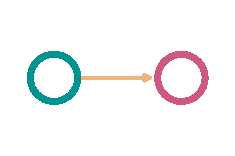
\includegraphics[width=\textwidth]{figures/point-to-point.pdf}
        \caption{Point-to-point}
        \label{fig:point-to-point}
    \end{subfigure}
    \hfill
    \begin{subfigure}[b]{0.22\textwidth}
        \centering
        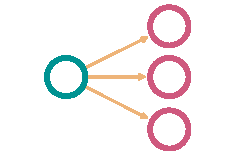
\includegraphics[width=\textwidth]{figures/isotropic-comm.pdf}
        \caption{Isotropic}
        \label{fig:isotropic}
    \end{subfigure}
    \hfill
    \begin{subfigure}[b]{0.22\textwidth}
        \centering
        \def\svgwidth{1\textwidth}
        \input{figures/anisotropic-comm.pdf_tex}
        \caption{Anisotropic}
        \label{fig:anisotropic}
    \end{subfigure}
    \hfill
    \begin{subfigure}[b]{0.22\textwidth}
        \centering
        \def\svgwidth{1\textwidth}
        \input{figures/coanisotropic-comm.pdf_tex}
        \caption{Co-anisotropic}
        \label{fig:co-anisotropic}
    \end{subfigure}
    
    \caption{Communication patterns in multiparty languages.}
    \label{fig:comm-patterns}
\end{figure}
These communication patterns provide a comprehensive set of primitives for expressing various communication scenarios in multiparty languages.

\subsection{Communication Operations in Other Languages}
To provide an overview of the communication operations supported by the selected DSLs,
\Cref{tab:comm-operations} summarizes the primitives provided by HasChor, CloudChor, ScalaLoci, and \ourLang{}.
%
\diff{We also include CloudChor~\cite{DBLP:conf/pepm/IonescuR26} as an internal DSL which, 
unlike the basic point-to-point interactions in HasChor, 
provides support for differentiated communication patterns.}
\begin{table}
    \centering
    \caption{Communication operations supported by multiparty languages.}
    \label{tab:comm-operations}
    \setlength{\extrarowheight}{2pt}
    \setlength{\tabcolsep}{3pt}
    \begin{tabularx}{\textwidth}{X c c l l}
        \hline
        \textbf{Comm. Types} & \textbf{HasChor} & \textbf{CloudChor} & \textbf{ScalaLoci} & \textbf{\ourLang{}} \\ \hline\hline
        Point-to-point       & \texttt{\textasciitilde>}        & \texttt{\textasciitilde>}   & \texttt{asLocal}*      & \code{comm}       \\ \hline
        Isotropic            & -  & \texttt{\textasciitilde>*}  & \texttt{asLocalFromAllSeq}*      & \code{isotropicComm}       \\ \hline
        Anisotropic          & -  & \texttt{\textasciitilde>.}  & \code{V per P on R}**      & \code{anisotropicComm}       \\ \hline
        Co-anisotropic       & -  & \texttt{*\textasciitilde>}  & \code{V per R on P}**      & \code{coAnisotropicComm}       \\ \hline
    \end{tabularx}
    \vspace{2pt}

    {\small * We considered the functions that trigger the communication.}\\
    {\small ** Differentiated communications are expressed at the type level.}
\end{table}
From the table,
we can see that HasChor only supports point-to-point communication,
meaning that if we want to support, for instance,
isotropic communication,
we need to manually provide the logic to send the same message to multiple receivers,
e.g., by invoking multiple point-to-point communications.
%
ScalaLoci,
on the other hand,
supports both point-to-point and isotropic communication,
allowing the receiver to extract the messages from all senders.
%
It also supports anisotropic and co-anisotropic communication,
however it requires boilerplate code to express these communication patterns,
as can be seen in the following example.
\begin{lstlisting}[style=scala3]
val deployTask: Signal[Task] per Worker on Master =
  { worker: Remote[Worker] => Signal { assocs().get(worker) }}
\end{lstlisting}
%
To express anisotropic communication in ScalaLoci,
developers must define a signal parameterized by the remote peer (\code{worker: Remote[Worker]})
and manually extract the appropriate message from an association map (\code{assocs().get(worker)}).
%
While flexible, this approach requires boilerplate code
and lacks the clarity of a dedicated communication primitive.
%
In contrast,
\ourLang{} provides native support for all communication patterns from \Cref{sec:comm-patterns}
through dedicated primitives,
simplifying multiparty coordination without sacrificing expressiveness.

\section{The \ourLang{} DSL}\label{sec:language}
Before introducing the characteristics of \ourLang{},
we present the main \emph{choreographic} and \emph{multitier} concepts that inspired our work.

\subsection{Type-level Architecture Definition}\label{sec:arch-def}
Having a clear and type-safe definition of the architecture of a distributed system is a fundamental aspect of \ourLang{}.
%
\diff{While several multiparty languages describe participants and communication structure in different ways,
our work adopts the explicit type-level architecture description introduced by ScalaLoci~\cite{DBLP:journals/pacmpl/WeisenburgerKS18},
where developers declare peer families together with their admissible communication ties.}
%
In \ourLang{},
\diff{we import this ScalaLoci-inspired architectural layer into a choreographic setting,}
allowing developers to define a set of peers and their communication relationships.
%
Inspired by ScalaLoci,
we defined an architecture with three peers: \texttt{Client}, \texttt{Server}, and \texttt{Database},
where the \texttt{Client} can communicate with the \texttt{Server},
and the \texttt{Server} can communicate with the \texttt{Database}.
%
\begin{lstlisting}[style=scala3]
// Clients (peer) can communicate with a single Server (tie relationship)
type Client <: { type Tie <: Single[Server] }
// Servers can communicate with a single Database and multiple Clients
type Server <: { type Tie <: Single[Database] & Multiple[Client] }
// Database can communicate with one Server
type Database <: { type Tie <: Single[Server] }
\end{lstlisting}
The architecture above specifies which \emph{class} of devices (i.e., peer types) are involved in the distributed system.
%
To declare \emph{instances} of these peers,
we use the \code{type Client} syntax as defined in the architecture.
%
To define \emph{connections} (i.e., which peer can communicate with which other peer),
we refine the peer definition specifying the \code{Client} to be a subtype (the \code{<:} in Scala refers to subtyping) of a structural type, i.e., an anonymous type with members defined inline,
enclosed in curly braces.
%
Such structural type defines a type member \code{Tie},
which specifies the communication relationships of the peer with other peers.
%
In the case of \code{Client},
the \code{Tie} type member is defined as \code{Single[Server]},
indicating that the \code{Client} can communicate with a single instance of \code{Server}.
%
When defining ties,
we can use the \emph{intersection type} operator \code{\&} to specify multiple communication relationships,
as shown in the definition of \code{Server}.
\subsubsection{Ties Relationships}
Leveraging the high flexibility of Scala's type system,
we can define the ``structural signature'' of a peer as \code{type Peer = \{ type Tie \}}.
%
Such a definition specifies a type alias to a structural type with a type member \code{Tie}.
%
However,
as such,
the \code{Tie} type member is unconstrained,
meaning that it can be defined arbitrarily.
%
Therefore, 
to impose constraints on the \code{Tie} type member,
we introduce two type constructors:
\begin{lstlisting}[style=scala3]
enum Quantifier[-P <: Peer]:
  case Single()
  case Multiple()
\end{lstlisting}
The \code{Quantifier} enum (i.e., an algebraic data type) introduces two type constructors: \code{Single} to denote a tie $\tieSingle{\pfam[1]}{\pfam[2]}$ where a peer is tied to a single instance of another peer,
and \code{Multiple} to denote a tie $\tieMult{\pfam[1]}{\pfam[2]}$ where a peer is tied to multiple instances of another peer.
%
However,
with this definition we are only describing the \emph{quantifier} of the tie relationship,
but we are not actually specifying which peer types are involved in the tie.

To overcome this limitation,
we introduced two types:
\begin{lstlisting}[style=scala3]
type TiedSingle[P <: Peer] = { type Tie <: Single[P] }
type TiedMultiple[P <: Peer] = { type Tie <: Multiple[P] }
\end{lstlisting}
The first one models a peer that is tied with a single instance of peer type \code{P},
while the second one models a peer that is tied with multiple instances of peer type \code{P}.
%
Such types are useful to express constraints on communication patterns between peers,
as we will see in the next sections.

\subsection{Placement Types}\label{sec:placement-types}
% \todo{The explanation of placement types and their runtime behavior (Section 4) could benefit from a brief intuitive summary to aid understanding. @Nicolas}
Both \emph{choreographic} and \emph{multitier} programming use the concept of ``values that live in the context of certain peer(s)'';
in the former,
it is often referred to as \emph{located values}
while in the latter, they are called \emph{placed values}.
%
Specifically,
at the type level,
we refine the value type with a notion of \emph{placement},
indicating where the value is located in the distributed system.

In \ourLang{},
we reuse the syntax from ScalaLoci to define placement types.
%
In Scala,
we can define a value of type \code{Int} that is placed at the \code{Client} peer as \code{Int on Client}.
%
The \code{on} type is an infix type which takes two type parameters:
the first is the base type (here, \code{Int}),
and the second is the peer where the value is placed (here, \code{Client}).

\diff{
Intuitively,
a value of type \code{V on P} should be read as ``a value of type \code{V} owned by peer \code{P}''.
%
When a multiparty program executes \code{on[P]},
only peers of type \code{P} actually evaluate the computation and materialize the value locally;
all other peers only keep a typed reference to that placed value.
%
As a consequence,
the value can be inspected with \code{take} only from within an \code{on[P]} context,
while communication primitives are the mechanism that makes the value available at other placements.}

Placement types are crucial in \ourLang{},
as they allow us to express where computations and data reside in the distributed system,
effectively encoding the peer instances $\epeer{n}{\pfam}$ of the runtime peer configuration $\peerconf$ (\Cref{def:arch-satisfaction}) at the type level.
In conjunction with the architecture definition,
they enable the type system to enforce communication constraints between peers.
%
This means that any attempt to communicate between peers not allowed by the architecture will result in a compile-time error,
thus preventing potential runtime failures due to invalid communications.

\subsection{Language Primitives}\label{sec:language-primitives}
\ourLang{} provides two categories of operations:
\textbf{placed computations} for defining peer-specific computations and extracting local values,
and \textbf{communication primitives} for peer-to-peer communication with differentiated schemes,
all enforcing architecture constraints at the type level.
These operations are defined in a single language trait, \code{MultiParty[F[_]: Monad]}, which abstracts over the effect type \code{F[_]}.
\diff{This trait requires a \code{Monad} constraint (via context bound syntax in Scala, namely \code{: Monad}) to support monadic composition and allow for various execution strategies, as detailed in \Cref{sec:implementation}.}
We now introduce the main primitives in detail.
%\todo{I'm a bit concerned that the names 'anisotropic'/'isotropic' might be a bit unintuitive to distributed systems people (maybe homogeneous and heterogeneous scatter/gather or something like that instead?). @All}

% As follow,
% we present the language primitives of \ourLang{} (\Cref{lst:language}),
% then in the next section,
% we discuss each primitive in detail.

% \begin{lstlisting}[
%     style=scala3,
%     caption={The \ourLang{} language trait defining the main primitives.},
%     label={lst:language}
% ]
% trait MultiParty[F[_]: Monad]:
%   type Remote[P <: Peer]
%   type Anisotropic[V]

%   def on[L <: Peer, V](body: Label[L] ?=> F[V]): F[V on L]
%   def take[L <: Peer](using Label[L])[V](placed: V on L): F[V]
%   def takeAll[Local <: Peer, V](
%     placed: Anisotropic[V] on Local
%   ): F[Map[Remote[Peer], V]]
%   def comm[S <: TiedSingle[R], R <: Peer, V](value: V on S): F[V on R]
%   def isotropicComm[S <: TiedMultiple[R], R <: TieWithSingle[S], V](
%     value: V on S
%   ): F[V on R]
%   def anisotropicMessage[S <: TiedMultiple[R], R <: TieWithSingle[S], V](
%     using Label[S]
%   )(value: Map[Remote[R], V], default: V): F[Anisotropic[V]]
%   def coAnisotropicComm[
%     From <: TiedSingle[To],
%     To <: TiedMultiple[From],
%     V
%   ](value: V on From): F[Anisotropic[V] on To]
%   def anisotropicComm[S <: TiedMultiple[R], R <: TieWithSingle[S], V](
%     value: Anisotropic[V] on S
%   ): F[V on R]
% \end{lstlisting}

\paragraph{Place and extract values.}
To define computations that execute on specific peers,
we need a mechanism to specify the execution context (the peer)
and a mechanism to access values placed at that context.
In \ourLang{},
these capabilities are provided by the following primitives:
\begin{lstlisting}[style=scala3]
trait MultiParty[F[_]: Monad]:
  def on[L <: Peer, V](body: Label[L] ?=> F[V]): F[V on L]
  def take[L <: Peer](using Label[L])[V](placed: V on L): F[V]
  /* ... other primitives ... */
\end{lstlisting}
Specifically, the \code{on} function executes computations only at peer instances of type \code{L}.
Its \code{body} parameter is a context function with an implicit \code{Label[L]} parameter,
enabling peer-specific operations like \code{take}.
The result is a placement type \code{V on L} wrapped in the effect \code{F[_]}.

%\paragraph{Extract placed value.}
The \code{take} function extracts values placed at peer type \code{L},
requiring an implicit \code{Label[L]} parameter available only within \code{on[L]} contexts.
This ensures that only locally placed values can be extracted;
attempting to extract remote values results in a compile-time error.

The following example demonstrates \code{on} and \code{take} together.
\begin{lstlisting}[style=scala3]
def example[F[_]: Monad](using MultiParty[F]): F[Int on Client] = for
  placedValue: String on Client <- on[Client] { "Hello, from Client!" }
  stringLength: Int on Client <- on[Client] { take(placedValue).map(_.length) }
yield stringLength
\end{lstlisting}
%The code abstracts over effect type \code{F[_]} constrained by \code{Monad},
%cleanly decoupling language specification from execution strategy (detailed in \Cref{sec:implementation}).
The \code{<-} operator acts as variable assignment in a monadic composition---namely, it is internally turned into a \code{flatMap} method call, namely, the bind monadic operation.
First, we place a string at \code{Client} producing \code{String on Client}.
Then, we extract it using \code{take}, compute its length, and place the result back at \code{Client}.

\paragraph{Point-to-point Communication.}
Following \Cref{def:point-to-point}, where a message $m$ is transmitted from a single sender $\epeer{}{P_s}$ to a single receiver $\epeer{}{P_r}$,
the \code{comm} function transmits values from source peer \code{S} to destination peer \code{R}.
\begin{lstlisting}[style=scala3]
trait MultiParty[F[_]: Monad]:
  /* ... other primitives ... */
  def comm[S <: TiedSingle[R], R <: TiedSingle[S], V](value: V on S): F[V on R]
\end{lstlisting}
The transmission is reflected in the type signature:
the input is a value placed at the sender \code{V on S}, and the result is a value placed at the receiver \code{V on R}---this type-level encoding is also used for the other communication primitives.
Crucially, this primitive enforces architectural compliance by constraining \code{S} and \code{R}
to be mutually tied to a single instance via \code{TiedSingle}.
\diff{
This primitive definition is similar to the one found in Choral~\cite{10.1145/3632398} and HasChor/CloudChor~\cite{10.1145/3607849}.}

To illustrate point-to-point communication,
consider a simple message exchange between two peers, \code{Alice} and \code{Bob}.
We assume these peers are defined in the architecture with a mutual single-instance tie relationship,
allowing them to exchange messages directly:
\begin{lstlisting}[style=scala3]
def pointToPointExample[F[_]: Monad](using MultiParty[F]): F[Unit] = for
  messageFromAlice <- on[Alice] { "Hello, Bob!" }
  messageAtBob <- comm[Alice, Bob](messageFromAlice)
  _ <- on[Bob]:
    take(messageAtBob).map(msg => println(s"Bob received: $msg"))
yield ()
\end{lstlisting}
% \todo{The comm primitive is strongly reminiscent (looks almost the same) as the one found in Choral [14]; that should be mentioned. @Nicolas}

\paragraph{Isotropic Communication.}
Recalling \Cref{def:isotropic},
isotropic communication sends the same message $m$ from one sender $\epeer{}{P_s}$ to all receiver instances $\{\epeer{1}{P_r}, \ldots, \epeer{n}{P_r}\}$---a
selective multicast to a specific peer class, distinct from indiscriminate broadcast.
\begin{lstlisting}[style=scala3]
trait MultiParty[F[_]: Monad]:
  /* ... other primitives ... */
  def isotropicComm[S <: TiedMultiple[R], R <: TiedSingle[S], V](v: V on S): F[V on R]
\end{lstlisting}
The function requires \code{S} tied to multiple \code{R} instances,
and \code{R} tied to a single \code{S} instance.

The following example shows the \code{Server} communicating with multiple \code{Client}s.
%
The \code{isotropicComm} function (line \ref{lst:isotropic-comm}) shares \code{updateFromServer} from \code{Server} to all \code{Client} instances.
%
Then,
each value is extracted in each client's context through \code{take} (line \ref{lst:isotropic-take}).
\begin{lstlisting}[style=scala3,escapechar=§]
def isotropicExample[F[_]: Monad](using MultiParty[F]): F[Unit] = for
  updateFromServer <- on[Server] { "Update available." }
  updateAtClients <- isotropicComm[Server, Client](updateFromServer)§\label{lst:isotropic-comm}§
  _ <- on[Client]:
    take(updateAtClients).map(update => println(s"Client received: $update"))§\label{lst:isotropic-take}§
yield ()
\end{lstlisting}

\paragraph{Anisotropic Communication.}
Corresponding to the pattern defined in \Cref{def:anisotropic},
anisotropic communication allows sending potentially different messages $m_i$ from a single sender $\epeer{}{P_s}$ to each receiver $\epeer{i}{P_r}$,
enabling per-receiver customization and reducing unnecessary communication overhead.
\begin{lstlisting}[style=scala3]
trait MultiParty[F[_]: Monad]:
  type Remote[P <: Peer]
  type Anisotropic[P <: Peer, V]
  /* ... other primitives ... */
  def anisotropicMessage[S <: TiedMultiple[R], R <: TiedSingle[S], V](
    using Label[S]
  )(value: Map[Remote[R], V], default: V): F[Anisotropic[R, V]]
  def anisotropicComm[S <: TiedMultiple[R], R <: TiedSingle[S], V](
    value: Anisotropic[R, V] on S
  ): F[V on R]
  def reachablePeers[R <: Peer]: F[NonEmptyList[Remote[R]]]
\end{lstlisting}
This pattern requires two functions:
\code{anisotropicMessage} creates an \code{Anisotropic[R, V]} value mapping remote instances to messages (with a default),
and \code{anisotropicComm} transmits it.
The \code{reachablePeers} function returns all reachable instances of a given peer type.
\diff{Together with the statically declared ties, this lets a choreography tailor messages to the concrete peer instances that are currently reachable and architecturally admissible.}

The following example shows \code{Server} sending different updates to \code{Client}s.
\begin{lstlisting}[style=scala3]
def anisotropicExample[F[_]: Monad](using MultiParty[F]): F[Unit] = for
  updates: Anisotropic[Client, String] on Server <- on[Server]:
    anisotropicMessage[Server, Client, String](
      reachablePeers[Client].map(client -> s"Update for $client").toMap,
      "No Updates"
    )
  updateAtClients <- anisotropicComm[Server, Client](updates)
  _ <- on[Client]:
    take(updateAtClients).map(update => println(s"Client received: $update")) 
yield ()
\end{lstlisting}
We create an anisotropic message mapping each \code{Client} to a custom update,
then transmit it via \code{anisotropicComm}.
Each \code{Client} extracts its specific update using \code{take}.

\paragraph{Co-anisotropic Communication.}
Dual to the anisotropic case (cf.\ \Cref{def:co-anisotropic}),
co-anisotropic communication captures the fan-in scenario
where
multiple senders $\{\epeer{1}{P_s}, \ldots, \epeer{n}{P_s}\}$ transmit potentially different messages $m_i$ to a single receiver $\epeer{}{P_r}$.
\begin{lstlisting}[style=scala3]
trait MultiParty[F[_]: Monad]:
  /* ... other primitives ... */
  def coAnisotropicComm[S <: TiedSingle[R], R <: TiedMultiple[S], V](
    value: V on S
  ): F[Anisotropic[S, V] on R]
  def takeAll[L <: Peer, R <: Peer](using Label[L])[V](
    placed: Anisotropic[R, V] on L
  ): F[Map[Remote[R], V]]
\end{lstlisting}
The \code{coAnisotropicComm} function collects messages from multiple \code{S} senders to a single \code{R} receiver,
producing \code{Anisotropic[S, V] on R}.
The \code{takeAll} function extracts individual messages as a map.
%
The following example shows multiple \code{Client}s sending to a single \code{Server}.
\begin{lstlisting}[style=scala3]
def coAnisotropicExample[F[_]: Monad](using MultiParty[F]): F[Unit] = for
  messageFromClient <- on[Client] { "Hello, Server!" }
  messagesAtServer <- coAnisotropicComm[Client, Server](
    messageFromClient
  )
  allMessages <- on[Server] { takeAll(messagesAtServer) }
  _ <- on[Server]:
    allMessages.foreach { case (client, msg) =>
      println(s"Server received from $client: $msg")
    }
yield ()
\end{lstlisting}
Each \code{Client} sends via \code{coAnisotropicComm},
and \code{Server} aggregates all messages using \code{takeAll}.

\section{Implementation}\label{sec:implementation}
\ourLang{} is implemented as an embedded DSL in Scala,
leveraging Scala's powerful type system and monadic abstractions to define the language semantics and execution model.
%
Its type system allows us to encode the architectural constraints and communication patterns at the type level,
ensuring that any architectural violation is caught at compile time,
while keeping the syntax clean and lightweight.

\subsection{Monadic Implementation}
Distributed systems inherently involve various computational effects:
network communication, asynchronous operations, error handling, and state management.
%
To ensure modularity and composability,
we adopt a monadic approach combined with the \emph{tagless final}~\cite{DBLP:journals/jfp/CaretteKS09} encoding style. %---an approach in which language constructs are represented not as data structures 
% (as in initial encodings or free monads) 
% but as methods of a type class (or trait) parameterized by an abstract type constructor \code{F[\_]}.
% %
% Programs are written against this abstract interface, 
% and concrete semantics are supplied by providing specific instances (interpreters) for \code{F[\_]}, 
% enabling multiple interpretations of the same program without modifying its definition.
Programs are parameterized by an abstract effect type \code{F[\_]},
with semantics defined purely through operations on this abstraction,
thereby decoupling language specification from concrete execution strategies.

This is particularly effective in multiparty scenarios where coordination primitives must compose seamlessly
regardless of whether they execute locally, communicate over the network, 
or involve other side effects.
%
In \ourLang{}, this translates to the \code{MultiParty[F[\_]]} trait,
whose primitives (e.g., \code{on}, \code{comm}, \code{isotropicComm}) are defined against the abstract effect \code{F[\_]}.
The bound \code{Monad} on \code{F[\_]} ensures that we can compose these operations in a monadic style, facilitating sequencing and error handling.
%
A production interpreter may instantiate \code{F} with \code{IO} backed by a real MQTT network,
while a test interpreter may substitute a pure, in-memory effect,
reusing the same program definition in both cases without modification.
%
Compared to free monads,
tagless final avoids the overhead of %constructing and interpreting an intermediate data structure,
% and simplifies the integration of additional effects
% without re-implementing the core language semantics for each new interpretation.
re-defining the language semantics for each interpreter,
reducing error-prone boilerplate and improving maintainability.
%
This design still ensures good testability---by allowing effect substitution for testing purposes---and
maintainability, as the language semantics is defined in a single place, independent of the execution strategy.

In practice,
the \code{MultiParty} effect is implemented by composing two lower-level effects:
\code{Network}, which abstracts the underlying communication layer,
and \code{Environment}, which encapsulates the peer's local execution context.
%
The \code{MultiParty} interpreter accepts these effect handlers as dependencies,
delegating network operations and context queries to them while orchestrating the high-level coordination logic.
%
%This compositional approach, enabled by tagless final encoding,
%allows each effect to evolve independently without tight coupling,
%facilitating modular testing and incremental enhancements to the runtime system.

\subsection{Placement Types}
The placement type implementation in \ourLang{} is rather straightforward,
as it is expressed as an infix type constructor \code{on} that takes a base type and a peer type as parameters.
%
Under the hood,
the \code{on} type is implemented as an \emph{algebraic data type} (ADT) with two type constructors:
\code{Local} which contains a unique identifier for the value placed,
and the value itself;
and \code{Remote} which contains only the unique identifier of the value placed.
%
Notably,
the unique identifier is a deterministic value that is used to reference the placed value in the distributed system.

A placement type is created out of a placed computation through the \code{on[P]} function.
%
At runtime,
when the \code{on[P]} function is evaluated,
the \code{P} peer is compared to the current peer type:
if they match,
the lambda body of the \code{on[P]} function is executed
and the resulting value is wrapped in a \code{Local} constructor;
otherwise,
the \code{on[P]} skips the execution of the lambda body and returns a \code{Remote} indicating that the value is not available locally.

Any operation that deals with a placement type checks whether the value is local or remote,
and acts accordingly.
%
For instance,
the \code{comm} function sends the value via network to the destination peer type \code{R} only if the value is local,
otherwise it interacts with the network to retrieve the value from the remote peer type \code{S}.
%
The general principle is very close to the one provided in~\cite{10.1145/3729296},
where the \emph{end-point-projection} (EPP) is performed at runtime.

\subsection{Network Layer}
The network layer is a dependency of the \code{MultiParty} interpreter,
abstracting the underlying communication mechanism and providing a uniform interface for sending and receiving messages between peers.
%
Its interface defines two main operations:
\begin{enumerate*}[label=(\roman*)]
  \item a \code{send} primitive that takes a message, its reference, and the destination peer type as parameters, and sends the message to the destination peer type;
  \item a \code{receive} primitive that takes a message reference and the source peer type as parameters, and waits for a message to be received from the source peer type with the given reference.
\end{enumerate*}
To complete the network layer,
we also need a primitive to retrieve the list of reachable peer instances of a given peer type,
and the local peer instance identifier.
\begin{lstlisting}[style=scala3]
trait Network[F[_], LP <: Peer]:
  type Address[P <: Peer]

  val localAddress: Address[LP]
  def send[V, To <: Peer](value: V, ref: Reference, to: Address[To]): F[Unit]
  def receive[V, From <: Peer](ref: Reference, from: Address[From]): F[V]
  def alivePeersOf[RP <: Peer: PeerTag]: F[NonEmptyList[Address[RP]]]
\end{lstlisting}
The network layer is intended as a (monadic) capability,
allowing a seamless integration with the \code{MultiParty} language---via the tagless final encoding---enabling multiple implementations of the network layer for different communication protocols like MQTT, HTTP, and gRPC.

% The network layer,
% even if from a first glance it may seem over simplified,
% is actually quite powerful and flexible,
Despite its simplicity,
the network layer ensures high flexibility and extensibility,
as we can implement \code{send} and \code{receive} primitives with different semantics (e.g., reliable vs unreliable, ordered vs unordered, etc.) and different underlying communication protocols,
providing specific guarantees to the layer above (i.e., the \code{MultiParty} interpreter).
%
The only constraint is imposed by the \code{alivePeersOf} primitive,
which must return a non-empty list of peer instances,
as the communication primitives in \ourLang{} assume that there is at least one reachable peer instance of the destination peer type.
%
This deals well with dynamic network topologies,
where peers can join and leave the network at runtime,
as the \code{alivePeersOf} primitive is implemented to reflect the current state of the network.
%
\diff{In this way, the static architecture fixes which peer families may communicate, while runtime peer discovery determines which concrete instances participate in each communication.}

\section{A taste of \ourLang{}}\label{sec:evaluation}

% \todo{- If the above is correct, you should reposition ScalaTropy as a choreographic programming language that imports the static architectural description features of ScalaLoci (which are peculiar to ScalaLoci, not multitier programming in general). I think your development shows that there is great advantage in doing so: you can implement pretty interesting patterns with your primitives that leverage architectural information at runtime. @Nicolas}
To assess the practical utility of \ourLang{}, we evaluate it across two dimensions: expressiveness, and communication overhead.
% \todo{In the evaluation section, it would be helpful to provide slightly more detail on the experimental setup. @Luca}

\subsection{Case Studies}

To showcase the expressiveness of \ourLang{} \diff{on} patterns \diff{studied in} both \diff{the ScalaLoci and choreographic programming literature},
we consider two representative examples: a Master-Worker application~\cite{DBLP:journals/pacmpl/WeisenburgerKS18} and a Replicated Key-Value Store~\cite{10.1145/3607849}.

\paragraph{Master-Worker application.}
We consider a Master-Worker application in which a Master peer dispatches tasks to multiple Worker peers,
and then aggregates the results to produce a final result (see \Cref{fig:master-worker}).
%
\begin{figure}[t]
\begin{lstlisting}[style=scala3]
object MasterWorker:
  type Master <: { type Tie <: Multiple[Worker] }
  type Worker <: { type Tie <: Single[Master] }

  case class Task(x: Int) { def compute: Int = x * x }

  def masterWorkerProgram[F[_]: MonadThrow](using MultiParty[F]): F[Unit] = for
    tasks <- on[Master]:
      for
        peers <- reachablePeers[Worker]
        allocation = peers.map(_ -> Task(Random.nextInt(100))).toList.toMap
        message <- anisotropicMessage[Master, Worker](allocation, Task(0))
      yield message
    taskOnWorker <- anisotropicComm[Master, Worker](tasks)
    partialResult <- on[Worker]:
      for
        t <- take(taskOnWorker)
        res <- t.compute.pure[F]
      yield res
    allResults <- coAnisotropicComm[Worker, Master](partialResult)
    result <- on[Master] { takeAll(allResults).map(_.values.sum) }
  yield ()
\end{lstlisting}
\caption{Master-Worker implementation in \ourLang{}.}
\label{fig:master-worker}
\end{figure}

From an architectural perspective, 
the \code{Master} peer is tied to multiple \code{Worker} peers,
  while each \code{Worker} peer is tied to a single \code{Master}.
%
% The \code{Task} case class represents the unit of work to be performed by the \code{Worker} peers---here the squaring of an integer for simplicity.
% %
% It derives \code{ReadWriter} to enable serialization for network transmission.
%
The application logic is implemented in the \code{masterWorkerProgram} function,
parameterized by an effect type \code{F[_]} constrained by \code{MonadThrow} to handle potential errors gracefully,
and a \code{MultiParty[F]} instance to access the language primitives.

Initially (lines 10-15), 
on the \code{Master} peer,
the reachable \code{Worker} peers are discovered;
%
a task is allocated to each, preparing an \emph{anisotropic message} for transmission.
%
Transmission is delegated to the \code{anisotropicComm} primitive,
which sends the corresponding task from the \code{Master} to each \code{Worker},
ensuring each \code{Worker} receives only its allocated task.
%
Next (lines 17-22),
on the \code{Worker} side,
the task is extracted, 
computed locally,
and the partial result is sent back to the \code{Master} using \code{coAnisotropicComm},
which collects the partial results into an anisotropic message placed on the \code{Master}.
%
By its semantics, \code{coAnisotropicComm} implements a barrier synchronization, blocking until all reachable \code{Worker} peers have computed and returned their results.
%
Finally (lines 24-26), the \code{Master} extracts all partial results and reduces them to produce the final result.

This program can be instantiated on a concrete peer instance, 
provided a network implementation and a coherent effect type as presented hereafter.

\begin{lstlisting}[style=scala3]
object MasterNode extends IOApp.Simple:
  override def run: IO[Unit] =
    val mqttNetwork = MqttNetwork
      .localBroker[IO, Master](Config(appId = "masterworker"))
    ScalaTropy(masterWorkerProgram[IO]).projectedOn[Master](using mqttNetwork)
\end{lstlisting}

\paragraph{Replicated Key-Value Store.}

The second example we considered is a Key-Value client-server application, where multiple clients interact with a remote key-value store, maintained by a server, supporting \code{put} (store) and \code{get} (retrieve) operations.
%
To ensure fault tolerance, the data store is replicated across multiple server instances, following a primary-backup replication scheme.
%
In this setup, clients communicate with a primary server instance for their operations, while the primary server is responsible for forwarding \code{put} operations to the backup server nodes to maintain data consistency across replicas.

The architecture of this system therefore consists of three peer types: \code{Client}, \code{Primary}, and \code{Backup}.
%
Each \code{Client} is tied to a single \code{Primary} server instance to which it sends its requests,
while the \code{Primary} server is tied to multiple \code{Backup} server instances and multiple \code{Client} peers.
%
\code{Backup} nodes are tied to a single \code{Primary} server instance from which they receive updates.
%
Responses and requests are encoded as ADTs as shown in the following code snippet.

\begin{lstlisting}[style=scala3]
object KeyValueStoreChoreo:
  type Client <: { type Tie <: Single[Primary] }
  type Primary <: { type Tie <: Multiple[Backup] & Multiple[Client] }
  type Backup <: { type Tie <: Single[Primary] }

  enum Request:
    case Get(key: String)
    case Put(key: String, value: String)
    case Empty

  enum Response:
    case Value(value: Option[String])
    case Ack
    case Empty
\end{lstlisting}

The code snippet in \Cref{fig:kvs} shows a synchronous implementation of the Key-Value client-server application: the \code{Primary} server applies writing operations, gathers acknowledgments from the \code{Backup} nodes, and then sends responses back to the clients.

\begin{figure}[t]
\begin{lstlisting}[style=scala3]
def kvs[F[_]: {Sync, Console}](
  primaryStorage: KeyValueStore[F, String, String] on Primary,
  backupStorage: KeyValueStore[F, String, String] on Backup,
)(using MultiParty[F]): F[Unit] = for
  requestOnClient <- on[Client](waitForRequest)
  requestsOnPrimary <- coAnisotropicComm[Client, Primary](requestOnClient)
  responsesOnPrimary <- on[Primary]:
    for
      store <- take(primaryStorage)
      requests <- takeAll(requestsOnPrimary)
      responses <- store processAll requests
      message <- anisotropicMessage[Primary, Client](responses, Empty)
    yield message
  putRequests <- on[Primary]:
    takeAll(requestsOnPrimary).map(_.values.collect { case r: Put => r })
  requestsOnBackups <- isotropicComm[Primary, Backup](putRequests)
  ack <- on[Backup]:
    for
      store <- take(backupStorage)
      requests <- take(requestsOnBackups)
      _ = requests.foreach(request => store process request)
    yield Ack
  _ <- coAnisotropicComm[Backup, Primary](ack)
  responseOnClient <- anisotropicComm[Primary, Client](responsesOnPrimary)
  _ <- on[Client]:
    take(responseOnClient) flatMap (response => F.println(s"> $response"))
  _ <- kvs(primaryStorage, backupStorage)
yield ()
\end{lstlisting}
\caption{Key-Value Store implementation in \ourLang{}.}
\label{fig:kvs}
\end{figure}

First, at line 5, \code{Client} peers wait for a request (coming from user's input or other sources).
%
Next, at line 6, each \code{Client} sends its request to the \code{Primary} server instance it is connected to, leveraging the \code{coAnisotropicComm} primitive.
%
Server-side, once all requests are received, they are unpacked, processed by the \code{Primary} server's local storage, and the corresponding responses are prepared for anisotropic communication back to the \code{Client} peers (lines 8-14).
%
Before sending, on the \code{Primary} server, all \code{Put} requests are extracted and forwarded to the \code{Backup} server instances using isotropic communication (lines 16-20).
%
This ensures each \code{Backup} node receives and consistently applies the client operations to its replica storage.
%
Finally, when all the \code{Backup} nodes have acknowledged the updates, the \code{Primary} server sends each response back to the corresponding \code{Client} using the \code{anisotropicComm} primitive (lines 22-24).
%
Computation continues recursively, 
allowing the system to process multiple requests over time.

By adopting an architectural definition, together with architecture-aware communication primitives,
the above implementation is guaranteed to work correctly with any number of backup replica servers.
%
In contrast, traditional choreographic implementations require the number of backup instances to be known in advance, 
and the communication logic to be explicitly defined for each instance.

\subsection{Selective Communication Advantages}
%\todo{In Section 5.2, you mention that 'simple choreographic approaches' wouldn't be as efficient. But your language is way more complicated, so it seems an unfair comparison. Don't we already have choreographic approaches that can do similar things, as in \url{https://doi.org/10.1007/978-3-319-39570-8_8}? This should be at least mentioned in related work. I actually think it'd make your paper stronger, since you offer an elegant implementation of some of the patterns therein. @Luca}

\ourLang{}'s support for selective communication primitives serves \diff{three} main purposes: 
(i) reducing unnecessary communication overhead, 
(ii) enhancing security by preventing information leakage to unintended recipients,
\diff{and (iii) providing richer expressiveness}.

\paragraph{Communication efficiency.}
Selective communication primitives enable the sender to transmit to each peer only the information that they require to accomplish their tasks.
%
This avoids the overhead associated with broadcasting messages to all participants and then filtering them at the receiver side, 
proving to be particularly beneficial in scenarios where the number of peers is large or when the total message size is significant.

To quantify the benefits of this approach, 
we consider a variant of the Master-Worker application discussed in \Cref{sec:evaluation},
for computing the matrix-vector product over large inputs.
%
This represents a canonical data-parallel workload,
where the Master partitions the matrix row-wise and distributes distinct row blocks to each Worker,
enabling independent computation of the corresponding partial results.
%
%Without selective communication primitives,
%like in simple choreographic programming approaches,
%the Master would broadcast the entire matrix to all Workers, 
%
\diff{By introducing a dedicated primitive for anisotropic communication, \ourLang{} avoids suboptimal communication patterns, such as broadcasting}
%
the entire matrix to all Workers, 
which would then filter out their relevant rows.
%---incurring significant 
%
This prevents significant communication overhead as the matrix size and number of Workers grow.
%
\Cref{fig:matrix-vector-evaluation} presents this communication overhead for a $50 \times 50$ \diff{representative} matrix, 
plotting the total data transmitted by the Master 
(or, equivalently, the cumulated data received by the Workers)
\diff{for the broadcast and the anisotropic communication approaches},
as the number of Workers increases.
%
\diff{
  Both were implemented in \ourLang{}, where the broadcast variant simply replaces \code{anisotropicComm} with \code{isotropicComm}, making them directly comparable within the same framework.
  %
  Data transmitted is measured in kilobytes (KB) at the network level; the results are independent of the underlying network protocol or deployment setup.
}
%approaches\footnote{
%   Both versions of the application were implemented in \ourLang{}; the broadcast variant simply replaces \code{anisotropicComm} with \code{isotropicComm}.
% }.
%
As expected, while the broadcast approach incurs a linear increase in communication overhead with the number of Workers,
the selective communication approach maintains almost constant overhead, with only a marginal increase due to per-Worker metadata and the distribution of the vector to be multiplied.

\begin{figure}[t]
  \centering
  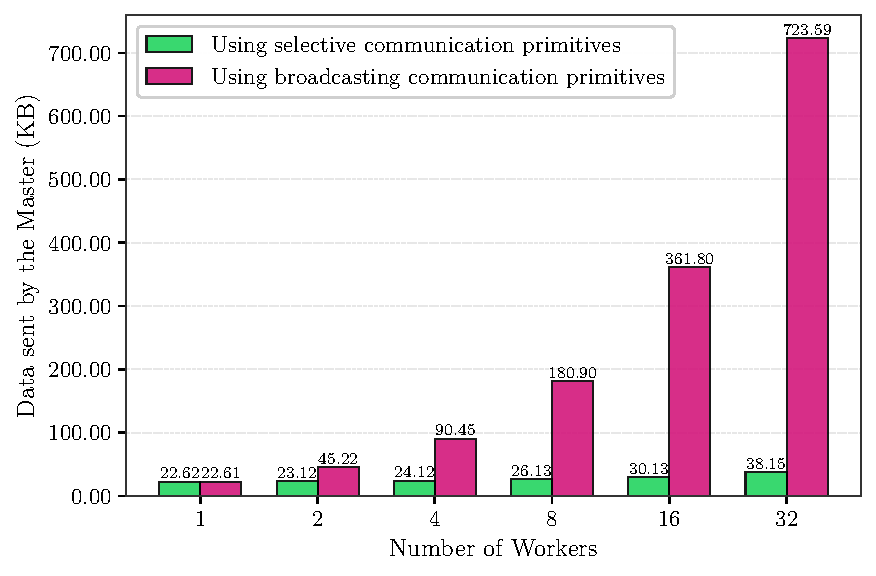
\includegraphics[width=0.9\textwidth]{figures/communication-overhead.pdf}
  \caption{Communication overhead comparison between broadcast and selective communication in a matrix-vector product application.}
  \label{fig:matrix-vector-evaluation}
\end{figure}

\paragraph{Security.}
%\todo{The security claim appears somewhat strong and is not fully supported; additional explanation or qualification would improve clarity. @Luca}
Beyond efficiency, selective communication primitives
%enable the principle of least privilege to be enforced 
\diff{contribute to data confidentiality} 
at the communication level:
%
\diff{
  by construction, each peer receives only the information necessary to perform its task,
  reducing the risk of unintended information disclosure compared to broadcast-based approaches.
}
%ensuring no information is leaked to unintended recipients when broadcasting sensitive data.

\paragraph{Expressiveness.}
Lastly, 
first-class support for selective communication patterns allows developers to express their intent more clearly in the code, 
avoiding 
%\diff{sending a separate point-to-point message per peer or} 
the opaque communication mechanisms required by existing multitier languages, 
such as the ScalaLoci pattern discussed in \Cref{sec:comm-patterns}.

\section{Related Work}\label{sec:related}
This work sits at the intersection of choreographic programming and multitier programming, 
 two paradigms that share the common goal of simplifying distributed system development through high-level abstractions.
%
Although session types represent a relevant line of research for multiparty communication,
 with several notable implementations such as Scribble~\cite{DBLP:conf/icdcit/HondaMBCY11}, Ferrite~\cite{chen_et_al:LIPIcs.ECOOP.2022.22}, 
 we do not discuss them in detail here, as our approach focuses on the integration of choreographic and multitier paradigms rather 
 than on session-typed communication channels.

\paragraph{Choreographic Programming.}
\sloppypar
Choreographic programming formalizes distributed coordination through global specifications~\cite{10.1145/2480359.2429101}.
%
On the practical side, the Jolie language~\cite{DBLP:books/sp/wsf14/MontesiGZ14} pioneered service-oriented coordination and influenced choreographic frameworks such as AIOCJ~\cite{dalla2017dynamic}, which supports safe runtime adaptation.
%
More recent implementations target specific host languages: Choral~\cite{10.1145/3632398} is a Java-based external DSL;
HasChor~\cite{10.1145/3607849} embeds choreographies in Haskell using monadic constructs;
and ChoRus~\cite{kashiwa2024chorus} brings choreographic programming to Rust.
%
These approaches primarily use point-to-point or broadcast communication, which can introduce overhead for selective multicast patterns.
%
\diff{Procedural Choreographies~\cite{CruzFilipe2017} formalizes this setting through a connection graph, while also supporting unbounded process creation and name mobility. In~\cite{CruzFilipe2016}, real-world computational algorithms are showcased using this language model.}
%
CloudChor~\cite{DBLP:conf/pepm/IonescuR26} extends HasChor with multicast primitives for selective dissemination but lacks architectural constraints.
%
Like HasChor and CloudChor, \ourLang{} uses monadic semantics for effect integration, but additionally enforces architectural constraints at the type level.

\paragraph{Multitier Programming.}
The Multi-Tier Calculus~\cite{10.1145/1040305.1040324} formalizes tier-crossing computations but provides no concrete implementation.
%
Practical languages include Ur/Web~\cite{10.1145/2775051.2677004}, Links~\cite{DBLP:conf/fmco/CooperLWY06}, and Hop~\cite{DBLP:conf/oopsla/SerranoGL06},
which unify client and server code but rely on implicit communication through shared placements.
%
ScalaLoci~\cite{DBLP:journals/pacmpl/WeisenburgerKS18} provides type-level architecture specification and enforcement, ensuring communications respect the declared architecture at compile time.
%
However, selective communication patterns in ScalaLoci require composition of lower-level primitives, 
which can increase syntactic overhead compared to dedicated first-class constructs.
%
\ourLang{} \diff{imports} ScalaLoci's \diff{type-level} architectural \diff{descriptions into a choreographic language} with explicit selective communication primitives.


\section{Conclusion}\label{sec:conclusion}
We presented \ourLang{},
\diff{a choreographic} language for multiparty coordination that \diff{integrates ScalaLoci-inspired architectural descriptions} in a single,
coherent framework.
%
We introduced explicit communication primitives for point-to-point, isotropic, anisotropic, and co-anisotropic communication patterns,
enabling developers to express their intent clearly and efficiently while ensuring architectural compliance through type-level constraints.
%
The monadic implementation of \ourLang{} allows for flexible execution strategies and seamless integration of effects,
while the placement type system ensures that values are accessed only in their intended contexts.

We evaluated \ourLang{} through representative case studies, demonstrating its expressiveness and efficiency in implementing common distributed coordination patterns.
%
Moreover,
we analyzed the communication overhead of selective communication primitives, showing their advantages over traditional broadcast approaches in terms of efficiency and security.

Future work includes formalizing the semantics of \ourLang{} and proving properties such as type safety and deadlock freedom,
as typical in the choreographic programming literature,
% \todo{This also begs for the question: could existing choreographic programming languages like Choral, HasChor, etc. borrow the lesson from this paper (have role instances and specify communications among roles, and then leverage runtime information about instances like you do)? It seems likely, so I'd point it out in future work. @Nicolas}
and architectural compliance and communication correctness for the ScalaLoci-inspired architectural layer adopted by the language.
\diff{Another direction is to investigate how existing choreographic languages such as Choral and HasChor could benefit from similar architectural descriptions and runtime role-instance information.}

%
% ---- Bibliography ----
%
% BibTeX users should specify bibliography style 'splncs04'.
% References will then be sorted and formatted in the correct style.
%
\nocite{*}
\bibliographystyle{splncs04}
\bibliography{bibliography}
%

% \newpage

% \appendix
% \section{Artefact Evaluation}

% \subsection{Badge claims}

% We claim two badges (i) \textbf{Available} and (ii) \textbf{Functional}.
% %
% The reasons why our artefact fulfils the requirements set out by the EAPLS scheme are outlined below.

% \subsubsection{Availability}

% The full code of the framework along with the case studies and the evaluation analysis
% is available as open source with a permissive license:

% \begin{itemize}
%   \item \emph{GitHub}: \href{https://github.com/nicolasfara/scalatropy}{\texttt{github.com/nicolasfara/scalatropy}}
%   \item \emph{Zenodo}: \href{https://zenodo.org/records/19407062}{\texttt{doi.org/10.5281/zenodo.19407062}}
% \end{itemize}

% \subsubsection{Functional outcomes}
% \begin{description}
%   \item[F1] The chart in \Cref{fig:matrix-vector-evaluation} shows the communication overhead of the selective communication primitives in \ourLang{} compared to a broadcast approach, demonstrating their efficiency advantages.
% \end{description}

% \subsection{Quick start}

% The artifact repository is structured as a single \code{mill} Scala project,
% with the following directory structure:
% \begin{description}
%   \item[\texttt{core}] contains the \ourLang{} implementation, including the language primitives, peer definitions, and the network layer abstraction;
%   \item[\underline{\texttt{examples}}] contains the case studies presented in \Cref{sec:evaluation}, including the Master-Worker application and the Replicated Key-Value Store, plus the matrix-vector product application used for the communication overhead evaluation, and a ping-pong example for testing purposes;
%   \item[\underline{\texttt{RunExperiments.sc}}] contains the code for running the communication overhead evaluation, which executes the matrix-vector product application with different numbers of Worker peers and measures the total communication overhead.
%   \item[\underline{\texttt{plot\_results.py}}] contains the code for plotting the results of the communication overhead evaluation, which generates the plot shown in \Cref{fig:matrix-vector-evaluation}. 
% \end{description}

% \subsubsection{Requirements}

% The artefact's evaluation is packed as a Docker image, including all necessary dependencies and configurations.
% %
% To run the evaluation, the following requirements must be met:
% %
% \begin{itemize}
%     \item \texttt{Docker} and \texttt{Docker Compose} installed on the machine;
%     \item sufficient computational resources to handle up to 32 concurrent \texttt{IOApp} instances of different parties. For example, the evaluation was performed on a machine with an 8-core CPU (6 performance and 2 efficiency cores), 16\,GB of RAM.
% \end{itemize}

% To speed up the evaluation process,
% the \texttt{sanity-checks.sh} script can be used to verify the presence of the necessary dependencies and tools to run the evaluation.
% %
% To perform the evaluation,
% the only mandatory requirement is to have Docker and Docker Compose installed on the machine, as the evaluation is packed as a Docker image that includes all the necessary dependencies and configurations.

% \subsection{Functional evaluation}

% To satisfy the functional claim \textbf{F1}, from the root of the project, it is sufficient to run:

% \begin{description}
%   \item \texttt{\$ docker compose up evaluation}
% \end{description}
% This downloads all the necessary requirements,
% builds the project,
% and runs the evaluation described in \Cref{sec:evaluation}.
% %
% % The whole experiment takes around five minutes to complete (not including the time to build the image and download the dependencies), and produces the communication overhead plot shown in \Cref{fig:matrix-vector-evaluation} inside the \texttt{evaluation} root project directory.
% The whole experiment may take from few minutes to around 20 minutes to complete, depending on the computational resources of the machine,
% and produces the communication overhead plot shown in \Cref{fig:matrix-vector-evaluation} at the path:%inside the \texttt{evaluation} root project directory.
% \begin{description}
%   \item \texttt{\$ ./evaluation/communication-overhead.pdf}
% \end{description}

% \subsection{Response to Reviewers}

% \subsubsection{Review 1}
% %
% The issue occurred because the reviewer's environment was unable to run 32 concurrent instances of the example on a single host.
% %
% This was due to the original evaluation setup, which required launching 33 autonomous peer instances (32 workers and 1 master) communicating via the MQTT broker.

% To ensure reproducibility without the computational overhead of spawning multiple JVM processes, the evaluation has been refactored to use an in-memory network spanning a single application.
% %
% Re-running 

% \begin{description}
%   \item \texttt{\$ docker compose up --build evaluation}
% \end{description}

% will now complete the evaluation significantly faster and without the previously encountered issues.

% \subsubsection{Review 2}
% %
% The discrepancies in \Cref{fig:matrix-vector-evaluation} were due to an inadvertent error in the manuscript preparation: the figure had been generated using an outdated version of the code prior to a refactoring step. 
% %
% The underlying conclusions were unaffected, and the figure has since been updated.
% %
% In case of acceptance, the updated figure will be included in the final version of the paper.

\end{document}
